\documentclass{beamer}

\usepackage[utf8]{inputenc}
\usepackage[T1]{fontenc}
\usepackage[english,russian]{babel}
\usepackage{amsmath}
\usepackage{amsfonts}
\usepackage{amssymb}
\usepackage{graphicx,pgf}
\usepackage{multimedia}
\DeclareMathOperator{\tr}{tr}
\usepackage{multirow}
\usepackage{subcaption}


%\usetheme{Copenhagen}
\usetheme{Warsaw}
\useinnertheme{circles}   %внутренняя тема
%\useoutertheme{smoothbars}   %внешняя тема
\usecolortheme{seahorse}     %цветовая схема
%\usefonttheme{serif}    %шрифты
%\defbeamertemplate*{footline}{shadow theme}
%\setbeameroption{hide notes}

%номера слайдов
\newcommand*\oldmacro{}%
\let\oldmacro\insertshorttitle%
\renewcommand*\insertshorttitle{%
	\oldmacro\hfill%
	\insertframenumber\,/\,\inserttotalframenumber}
\RequirePackage{caption}
\DeclareCaptionLabelSeparator{defffis}{ }
\captionsetup{justification=centering,labelsep=defffis}

%\title{Курсовая работа}
%\subtitle{Численные схемы для аппроксимации неограниченных решений при моделировании обтекания профиля крыла в вихревых методах}
\title[Моделирование термоупругого ...]{Математическое моделирование термоупругого разрушения хрупкого материала}
\author[Швецов Г.А.]{Докладчик: Швецов Г.А.\and\\[0.5mm] Научный руководитель: д.ф-м.н., профессор кафедры ФН-2 Галанин М.П.}

\institute[каф. Прикладная математика ФН-2]{группа ФН2-52Б}
\date{\today}
\titlegraphic{
\includegraphics[width=1.8cm]{logo.png}}
%\renewcommand{\vec}[1]{\text{\mathversion{bold}${#1}$}}

\begin{document}
		\newcommand{\pl}{\partial}
	\begin{frame}
		\titlepage
	\end{frame}
			
	\begin{frame}{Постановка задачи. Цель}
		\begin{block}{Цель}
			Цель работы -- построение и анализ одномерной модели разрушения стержня, а также решение задачи термоупругости разностной схемой и нахождение аналитического решения для линейного случая.
		\end{block}
		\begin{block}{Постановка задачи}
			\footnotesize
			\begin{enumerate}
				\item Тензор малых деформаций Коши
				\[
				\varepsilon_{kl} = \dfrac{1}{2}\Bigl( \dfrac{\partial u_k}{\partial x_l} + \dfrac{\partial u_l}{\partial x_k} \Bigr) = \varepsilon_{kl}^e +  \varepsilon_{kl}^0, \quad \varepsilon_{kl}^0 = \varepsilon_{kl}^T=\alpha_{kl}^T \Delta T.
				\]
				\item Обобщенный закон Гука
				\[
				\sigma_{ij} = C_{ijkl} \varepsilon_{kl}^e = C_{ijkl}(\varepsilon_{kl} - \varepsilon_{kl}^0).
				\]
				\item Уравнения равновесия
				\[
				\dfrac{\partial \sigma_{ji}}{\partial x_j} + b_i = 0.
				\]
			\end{enumerate}
		\end{block}
	\end{frame}
	
	\begin{frame}{Модель размазанных трещин}
	\begin{block}{Аппроксимация}
	\begin{equation}
	\dfrac{\sigma}{\sigma_f} = A + B e^{-C \tfrac{\varepsilon}{\varepsilon_f}},	
	\end{equation}
	где коэффициенты A, B выводятся экспериментально.\\ Для дикосида урана UO$_2$:
	$
	A = -0.024,\, B = 1.69, \, C = 0.5.  
	$
	\end{block}
	\begin{figure}[h]
	\centering
	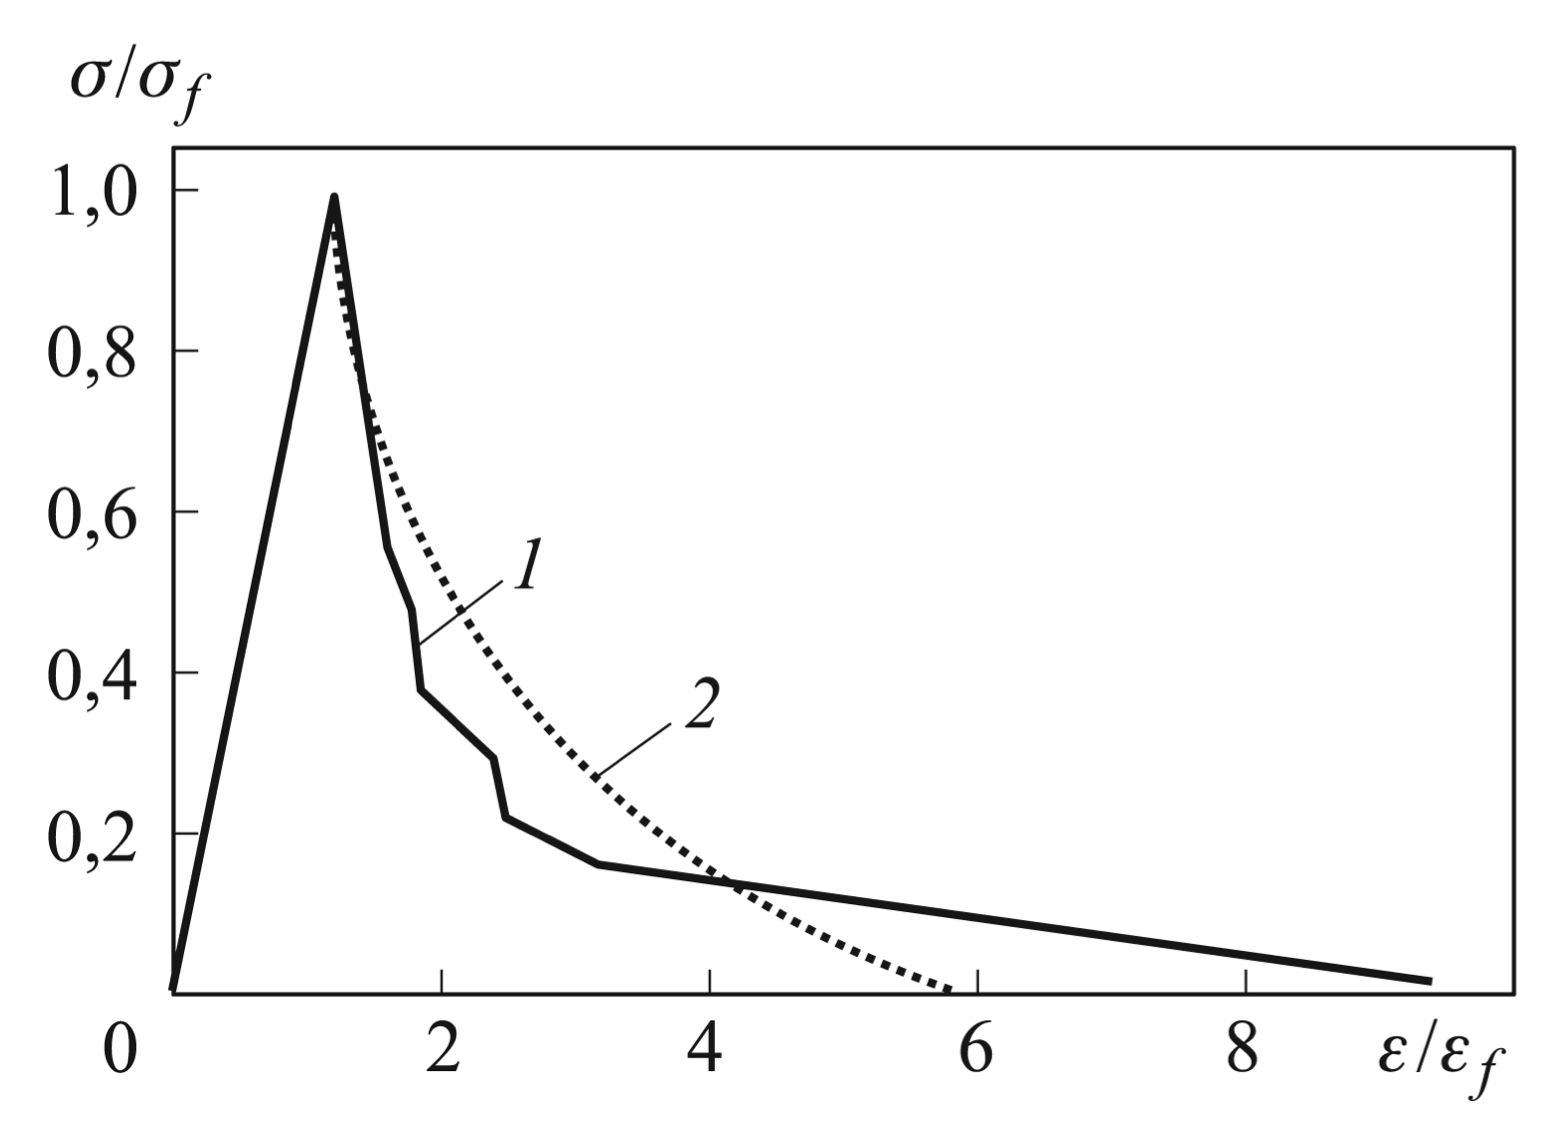
\includegraphics[width=0.53\textwidth]{ceramic}
%	\captionsetup{labelformat=empty}
		\caption{\small{Экспериментальная (1) и аналитическая (2) кривые растягивающего отклика для керамических материалов}}
%	\caption{Экспериментальная (1) и аналитическая (2) кривые нормализованного растягивающего отклика для керамических материалов}
	\label{fig:ceramic}
\end{figure}
	\end{frame}
	
	\begin{frame}{Одномерный случай}
	\begin{block}{Зависимость напряжений от деформаций}
	\begin{equation}
	\sigma(\varepsilon) = 
\begin{cases}
	E\varepsilon^e, & E\varepsilon^e < \sigma_f^v(\varepsilon), \\
	\sigma_f^v(\varepsilon),\,\sigma_f^v= \sigma_f\Bigl( A + B e^{-C \tfrac{\varepsilon-\varepsilon^T}{\varepsilon_f}} \Bigr), & E\varepsilon^e \geq \sigma_f^v(\varepsilon),
\end{cases}
\label{sigma}
	\end{equation}
\noindent где $\sigma_f^v(\varepsilon)$ -- переменный предел прочности ($\sigma_f^v(0) = \sigma_f$).
		\begin{equation}
\varepsilon^e = \varepsilon - \varepsilon^T-\varepsilon^{crk},
\end{equation}
		\begin{equation}
\varepsilon^{crk} = \varepsilon-\varepsilon^T-\frac{\sigma(\varepsilon)}{E},
	\end{equation}
где $\varepsilon^e$ -- упругие деформации, $\varepsilon^{crk}$ -- деформации за счет трещин, $\varepsilon^T$ -- температурные деформации, $E$ -- модуль Юнга.
\end{block}
	\end{frame}
	
		
	
	\begin{frame}{Математическая модель для стержня}
		\begin{block}{Знакопеременная нагрузка за счет изменения температуры}
\[
T(x,t) = \tilde T+F(x)\tau(t),
\]
где $F(x)$ -- пространственное распределение температуры,\\  $\tau(t)$ -- временн\'{о}е, $\tilde T$ -- усредненная по времени температура.
		\end{block}
		
		\begin{block}{Одномерная модель}
			\[
			\begin{cases}
				T(x, t) = \widetilde{T} + F(x) \tau(t), & t \geq 0, \quad 0 \leq x \leq l, \\[0.7em]
				\sigma = \sigma(\varepsilon - \varepsilon^T), & \varepsilon = \dfrac{\partial u}{\partial x}, \quad \varepsilon^T = \alpha(T - T_0), \\[0.7em]
				\dfrac{\partial \sigma}{\partial x} = 0, & 0 \leq x \leq l, \\[0.7em]
				u(0, t) = u(l, t) = 0.
			\end{cases}  
			\]
			
		\end{block}
	\end{frame}
	
	\begin{frame}{Тестовая задача}
		\mbox{Пусть $F(x) = a \sin\left(\frac{\pi x}{l}\right), \tau(t) = t\sin(t), a = 50, T_f = 20 \text{ c}, l=10,$}\\$\tau_h = 0.005\text{ c}, T_0 = \tilde T=300\text{ К,} n=10.$
		
		 Для упругого случая составим дифференциальное уравнение и найдем аналитическое решение.
		\begin{block}{Линейный случай}
		\begin{gather*}
			\sigma(\varepsilon) = E\varepsilon^e=E(\varepsilon-\varepsilon^T)=E\left(\frac{\pl u}{\pl x}-\alpha(T(x,t)-T_0)\right),\\
			\frac{\pl \sigma}{\pl x} = 0 \quad \Leftrightarrow \quad \frac{\pl^2u}{\pl x^2} = \alpha \frac{\pl T(x,t)}{\pl x}.
		\end{gather*}
	\end{block}
	\begin{block}{Аналитическое решение}
			\[
			u(x, t) = \alpha\frac{ a t \sin(t)}{\pi}\left(l-2x-l\cos\left(\frac{\pi x}{l}\right)\right).
			\]
		\end{block}
	\end{frame}
	
	\begin{frame}{Зависимость напряжения $\sigma$ от деформаций $\varepsilon-\varepsilon^T$}
		\begin{figure}[H]
			\centering
			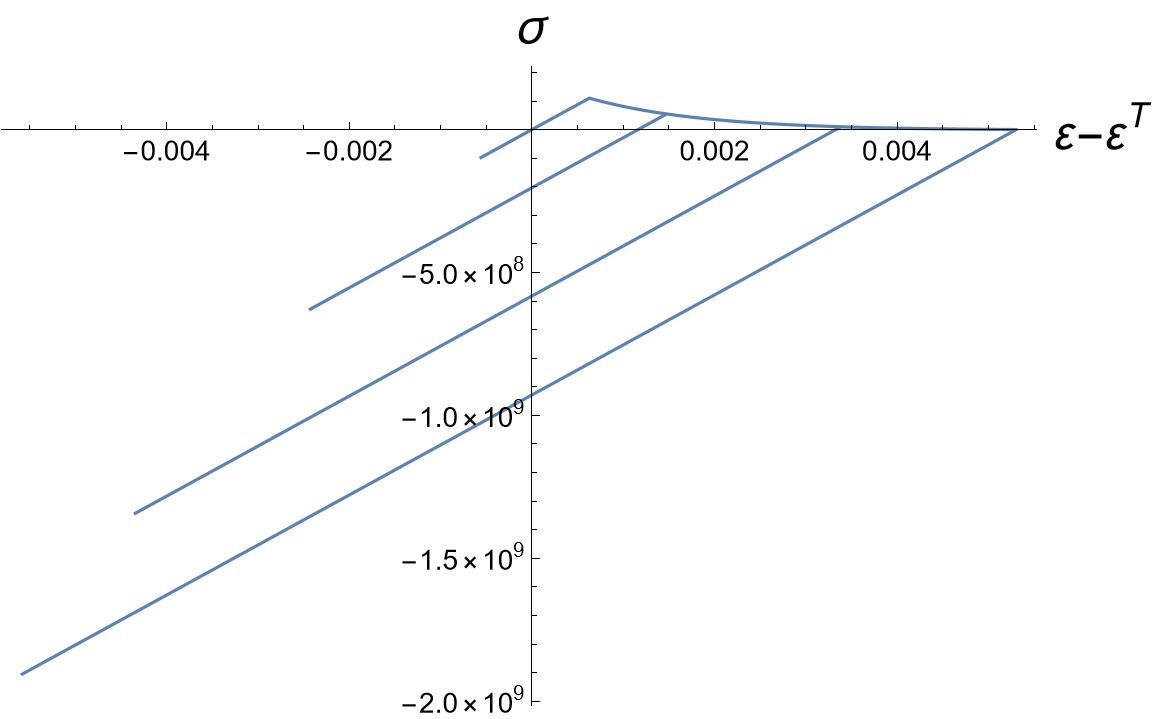
\includegraphics[width=1\textwidth]{T1_4}
		\end{figure}
	\end{frame}
	
	\begin{frame}{Зависимость $\varepsilon$, $\varepsilon^{crk}$, $T$ от $t$}
	\begin{figure}
		\begin{minipage}{0.45\textwidth}
			\center{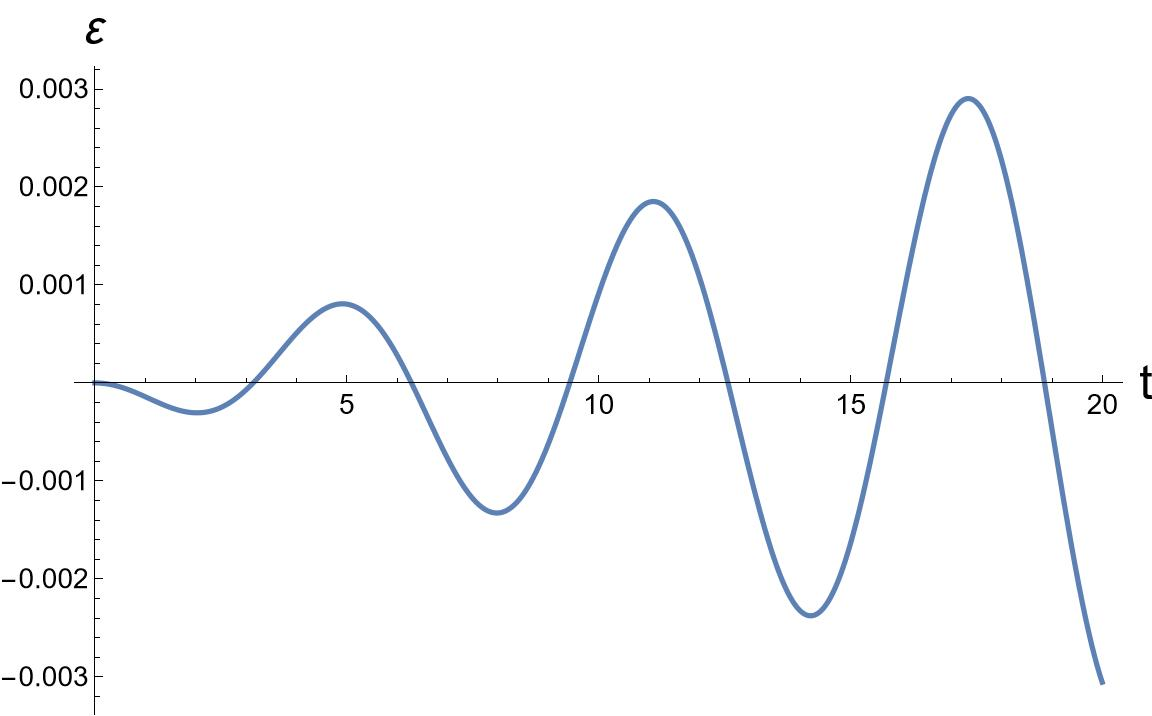
\includegraphics[width=\textwidth]{T1_1}}
		\end{minipage}
		\hfill
		\begin{minipage}{0.45\textwidth}
			\center{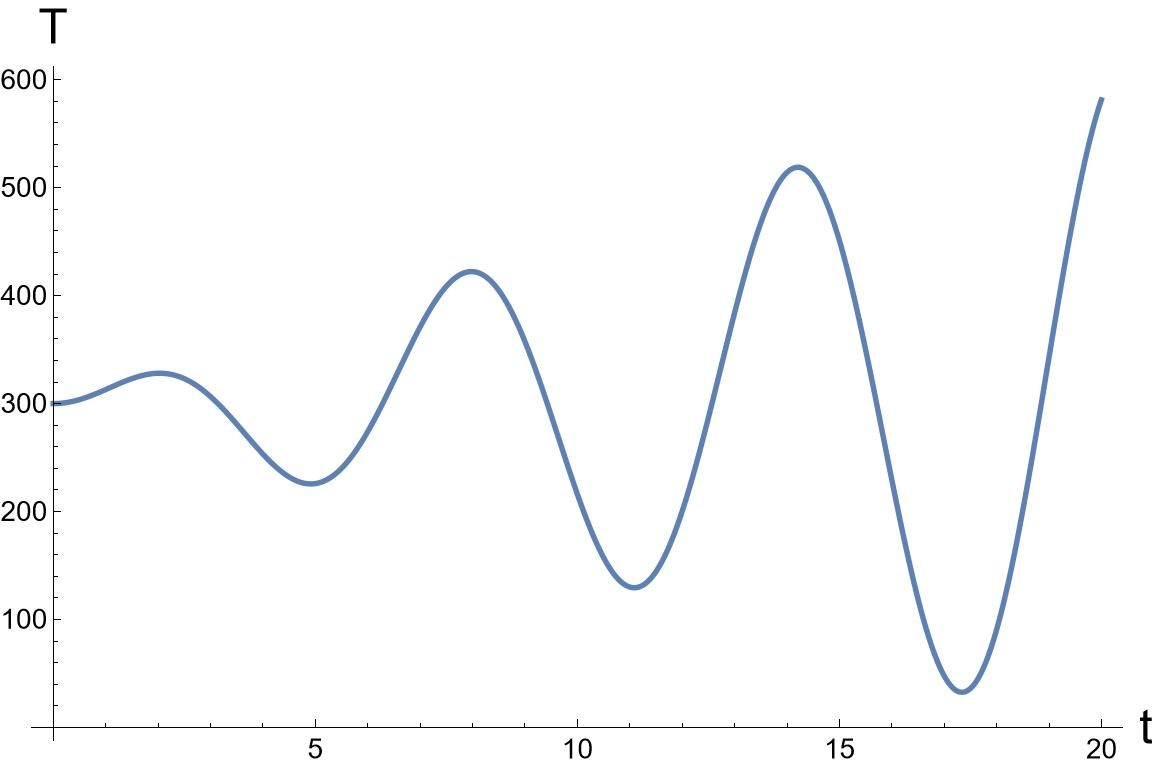
\includegraphics[width=\textwidth]{T1_6}}
		\end{minipage}
		\label{ris:image1}
	\end{figure}
\begin{figure}
	\centering
	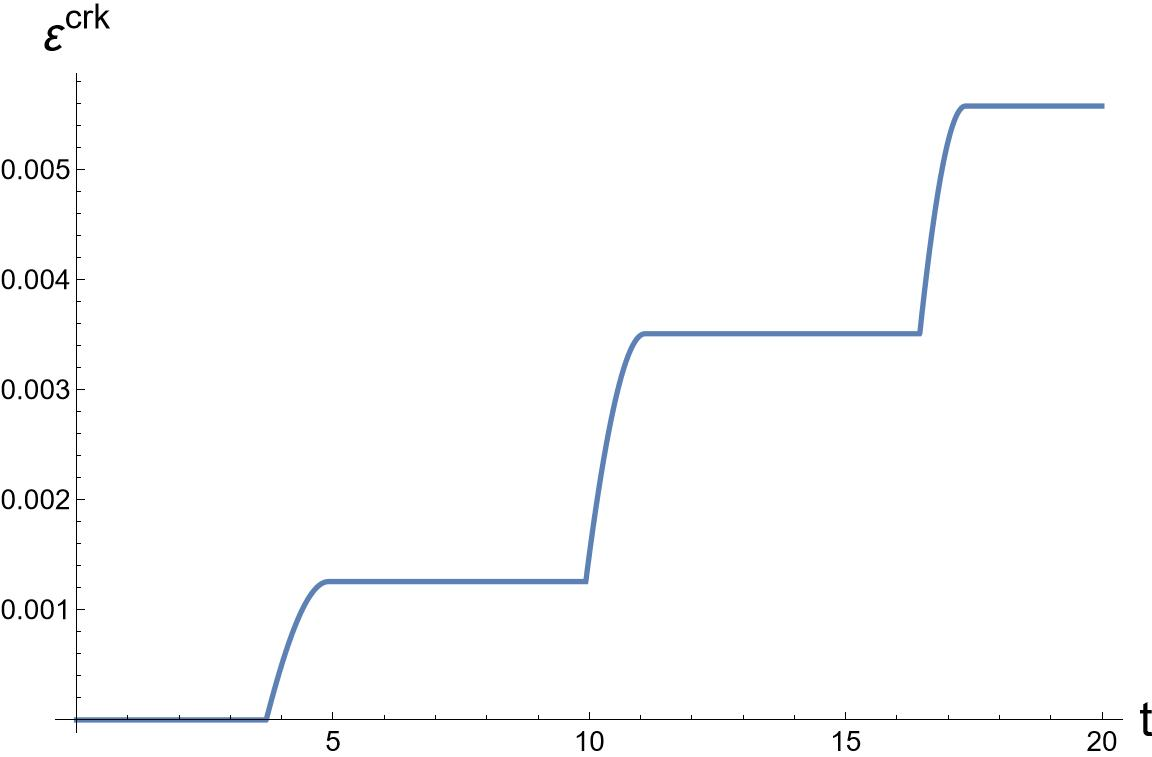
\includegraphics[width=0.5\textwidth]{T1_2}
\end{figure}
	\end{frame}

\begin{frame}{Зависимость $\sigma$ от $t$ }
	\begin{figure}[H]
	\centering
	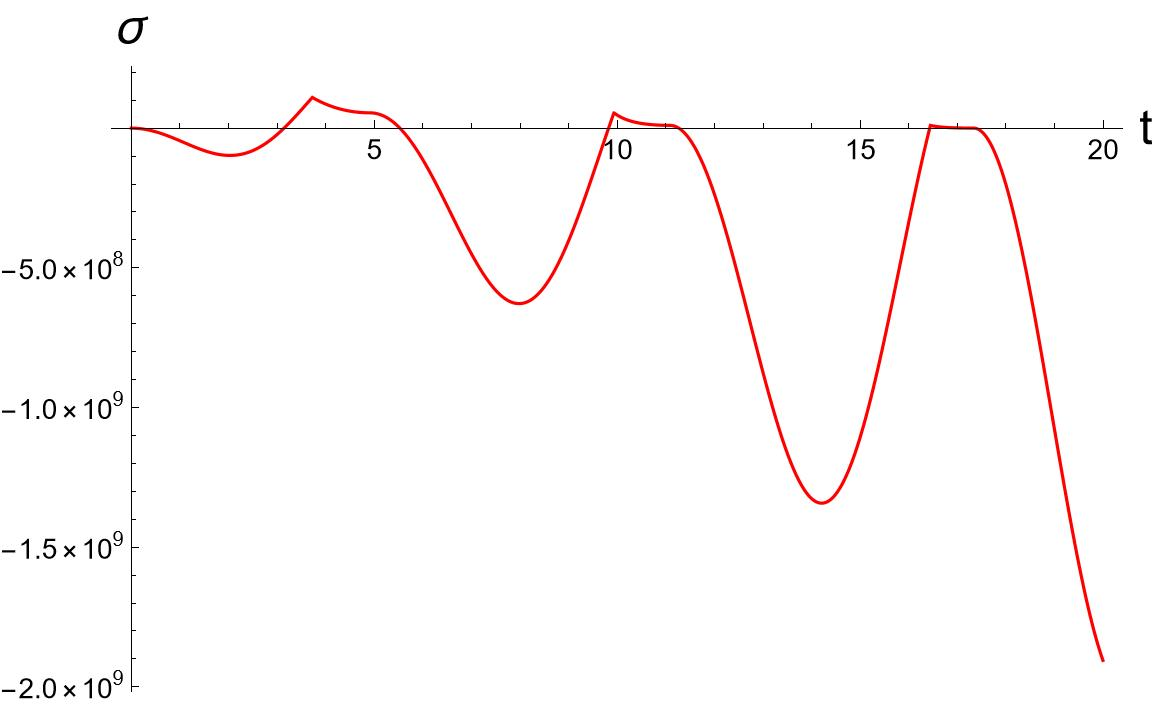
\includegraphics[width=1\textwidth]{T1_3}
\end{figure}
\end{frame}
	
	\begin{frame}{Заключение}
		\begin{enumerate}
			\Large
			\item Построена математическая модель разрушения стержня в одномерном случае;
			\item Методом конечных разностей на равномерной сетке решена задача термоупругости;
			\item Для линейного случая найдено аналитическое решение.
		\end{enumerate}
	\end{frame}
	
	
	\begin{frame}
		\frametitle{Список использованных источников}
		\begin{thebibliography}{9}
				
			\bibitem{galanin1} \textit{Галанин М.П., Савенков Е.Б.} Методы численного анализа математических моделей. М.: Изд-во МГТУ им. \mbox{Н.Э. Баумана},	2010. -- 592 с.
			
			\bibitem{galanin2} Математическое моделирование разрушения хрупкого материала под действием тепловых нагрузок / М.П. Галанин [и др.] // Препринты ИПМ им. М.В. Келдыша. 2013.No 100. -- 36 с. URL: \url{http://library.keldysh.ru/preprint.asp?id=2013-100}
		
			\bibitem{frost} \textit{Фрост Б.} ТВЭЛы ядерных реакторов: пер. с англ. М.: Энергоатомиздат, 1986. --
			\mbox{248 с.}
			\bibitem{zarubin} \textit{Зарубин В.С., Кувыркин Г.Н.} Математические модели механики и электродинамики сплошной среды. -- М.: Изд-во МГТУ им. Н.Э. Баумана, 2008. -- 512 с.: ил. (Математическое моделирование в технике и в технологии).
		
		\end{thebibliography}
	\end{frame}

\begin{frame}
\LARGE
\centering
Спасибо за внимание!
\end{frame}
	
	
	
\end{document}